\chapter{Architecture for Reliable Agent Systems}
Reliable agent systems combine orchestration, state, tools, evaluation, and policy. LangChain is helpful for linear chains and tool wrappers. LangGraph becomes important when the system needs durable state, branching, retries, and human-in-the-loop decisions. CrewAI is especially natural when the mental model is organizational work: a crew of agents coordinating through tasks and context.

\section{A Simple Reliability Model}
A compact way to reason about production readiness is to combine task success, verification coverage, and control strength while subtracting risk exposure:
\[
R = \alpha S + \beta V + \gamma C - \delta E
\]
where $S$ is measured success rate, $V$ is verification coverage, $C$ is control maturity, and $E$ is exposure caused by risky tools or permissions. The formula is intentionally simple: it reminds engineers that model quality alone cannot carry a production system.

\begin{figure}[h]
\centering
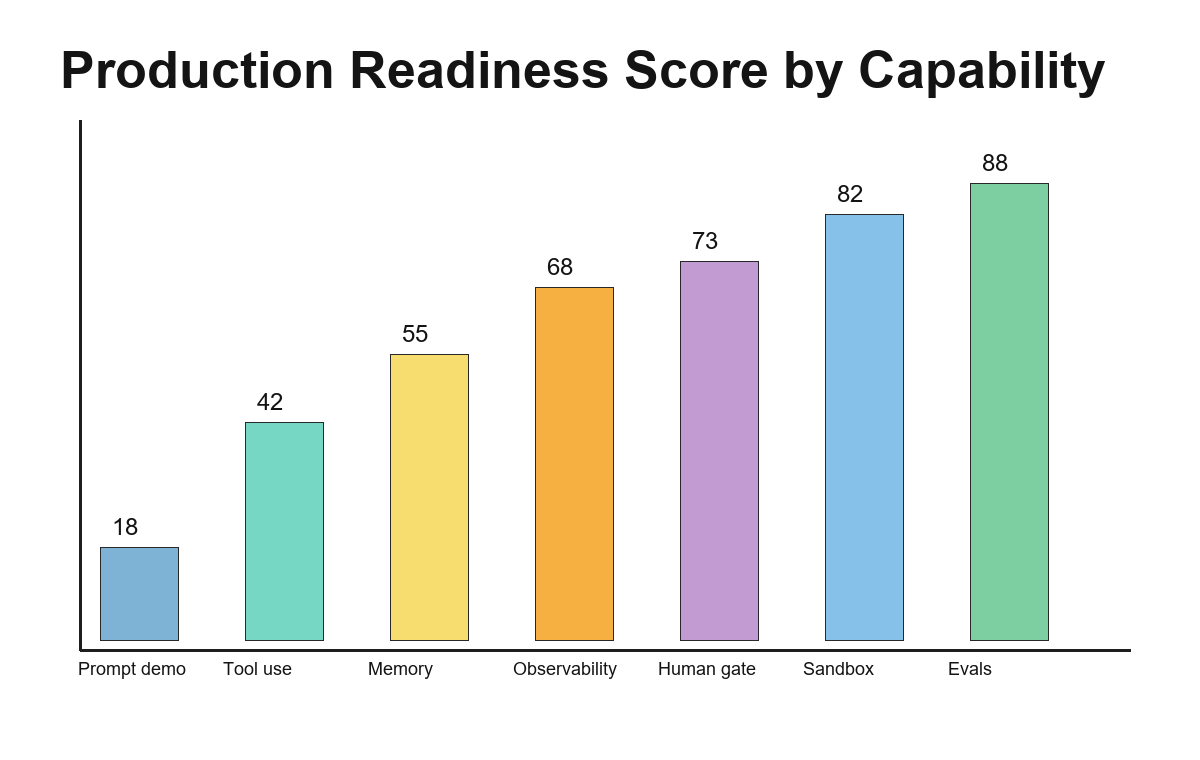
\includegraphics[width=0.88\textwidth]{assets/readiness_chart.png}
\caption{Python-generated chart showing readiness gains as controls are added.}
\end{figure}
